% ============================================================
% 数电实验报告
% ============================================================

\documentclass[12pt]{ctexart}

% --- 宏包 ---
\usepackage{graphicx}
\usepackage{amsmath}
\usepackage{listings}
\usepackage{float}
\usepackage{booktabs}
\usepackage{siunitx}
\usepackage{fancyhdr}
\usepackage{caption}
\usepackage{subcaption}
\usepackage{hyperref}
\usepackage{makecell}
\usepackage{enumitem}

\sisetup{per-mode=symbol}

\graphicspath{{./figures/}{../figures/}}

\usepackage[left=2.5cm, right=2.5cm, top=2.5cm, bottom=2.5cm]{geometry}

\setlength{\jot}{6pt}
\setlength{\headheight}{15pt}
\linespread{1.5}
\setlist{nosep}

% --- 页眉页脚 ---
\pagestyle{fancy}
\fancyhead[C]{数字电子技术实验}
\fancyfoot[C]{\thepage}

\begin{document}

% ==================== 封面 ====================
\thispagestyle{empty}

\begin{figure}[t]
    \centering
    
\includegraphics[width=13cm]{logo1.png}
\end{figure}

\vspace*{\fill}
    \begin{center}
        \Huge\textbf{数字电子技术基础}

        \vspace{0.3cm}
        \Huge\textbf{实验报告}

        \vspace{1cm}
        \LARGE\textbf{实验二：组合逻辑电路设计}
    \end{center}
\vspace*{\fill}

\begin{table}[H]
    \centering
    \large
    \begin{tabular}{ll}
    \toprule
    \textbf{课程:} & 数字电子技术实验 \\
    \textbf{组员1:} & 郭浩然 2024303980 \\
    \textbf{组员2:} & 庞铭洋 2024302539 \\
    \textbf{组号:} & 15 \\
    \textbf{时间:} & \today \\
    \bottomrule
    \end{tabular}
\end{table}

\newpage

% ==================== 正文 ====================

\section{实验目的}

\begin{enumerate}
    \item 掌握利用中规模集成组合逻辑器件实现组合逻辑电路的方法。
    \item 学习使用 74153 双四选一数据选择器和 7400 与非门设计一位全减器。
    \item 学习使用 74138 三线八线译码器和与非门设计密码锁电路。
    \item 掌握在 Quartus II 中采用原理图输入、波形仿真、引脚分配和 FPGA 下载验证的基本流程。
    \item 理解多个组合逻辑模块之间的联动控制方法，能够实现密码正确时全减器正常工作的综合功能。
\end{enumerate}

\section{实验要求}

\begin{enumerate}
    \item 使用组合逻辑器件 74153 双四选一数据选择器和 7400 与非门，用原理图输入方法实现一位全减器。
    \item 使用组合逻辑器件 74138 三线八线译码器和与非门，用原理图输入方法实现一个密码锁。密码设为 \texttt{1111}，当密码输入正确时 LED 点亮。
    \item 将密码锁与全减器连接，使密码正确时全减器正常工作；密码错误时，全减器输出被禁止或不表示有效运算结果。
    \item 使用 Quartus II 完成原理图输入、波形仿真，并将设计下载到 DE0 开发板进行验证。
\end{enumerate}

本组两名组员学号最后一位分别为 0 和 9，其四位二进制表示分别为 \texttt{0000} 和 \texttt{1001}；密码正确状态为 \texttt{1111}。

\section{实验设备}

\begin{itemize}
    \item Quartus II 开发软件
    \item DE0 开发板（FPGA 型号：Cyclone V 5CEBA4F23C7）
    \item USB-Blaster 下载线及计算机
    \item 组合逻辑器件符号：74153、74138、7400 及相关输入输出引脚
\end{itemize}

\section{实验原理}

\subsection{一位全减器}

一位全减器用于完成被减数 $A$、减数 $B$ 和来自低位借位 $C_i$ 的一位二进制减法运算，输出差位 $D$ 和向高位借位 $C_o$。其逻辑关系为
\begin{align}
    D &= A \oplus B \oplus C_i, \\
    C_o &= \overline{A}B + \overline{A}C_i + BC_i.
\end{align}

一位全减器真值表如表~\ref{tab:sub_truth} 所示。

\begin{table}[H]
    \centering
    \caption{一位全减器真值表}
    \label{tab:sub_truth}
    \begin{tabular}{ccc|cc}
        \toprule
        $A$ & $B$ & $C_i$ & $D$ & $C_o$ \\
        \midrule
        0 & 0 & 0 & 0 & 0 \\
        0 & 0 & 1 & 1 & 1 \\
        0 & 1 & 0 & 1 & 1 \\
        0 & 1 & 1 & 0 & 1 \\
        1 & 0 & 0 & 1 & 0 \\
        1 & 0 & 1 & 0 & 0 \\
        1 & 1 & 0 & 0 & 0 \\
        1 & 1 & 1 & 1 & 1 \\
        \bottomrule
    \end{tabular}
\end{table}

74153 为双四选一数据选择器，每个数据选择器有两个地址输入和四个数据输入。将变量 $A$、$B$ 作为选择端，把 $C_i$ 或其反变量按真值表接入数据端，即可分别实现差位 $D$ 和借位 $C_o$ 的逻辑函数；再配合 7400 与非门产生所需的反相信号和控制逻辑。

\begin{figure}[H]
    \centering
    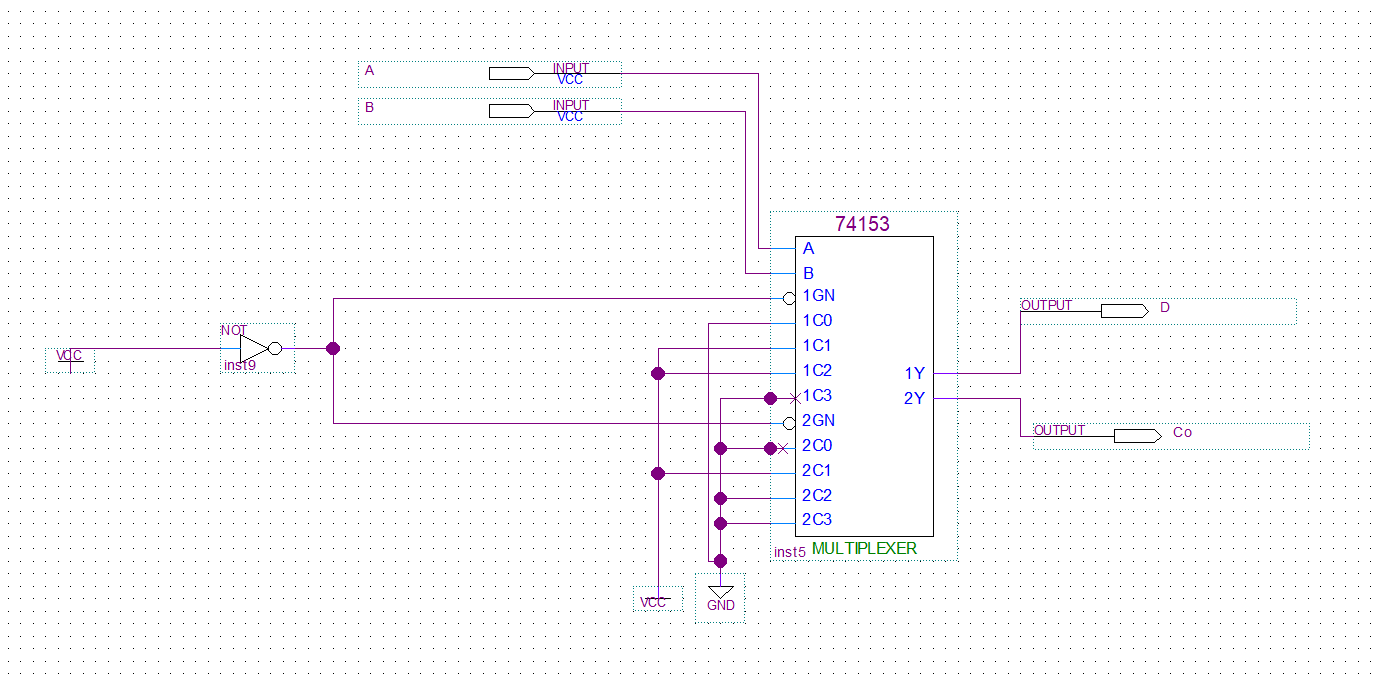
\includegraphics[width=0.95\textwidth]{减法器电路.png}
    \caption{基于 74153 和 7400 的一位全减器原理图}
    \label{fig:sub_circuit}
\end{figure}

\subsection{密码锁电路}

密码锁电路使用 74138 三线八线译码器实现输入状态识别。74138 在使能有效时，根据三位输入选择一个低有效输出端。由于实验密码为 \texttt{1111}，可将四位密码输入拆分为译码输入和使能控制：当高位条件和低三位译码结果同时满足时，通过与非门组合得到密码正确标志信号。

对于本组输入，学号末位 0 和 9 可分别表示为 \texttt{0000} 和 \texttt{1001}。实验中以 \texttt{1111} 作为密码正确状态，并用 LED 显示密码锁判断结果。

\begin{figure}[H]
    \centering
    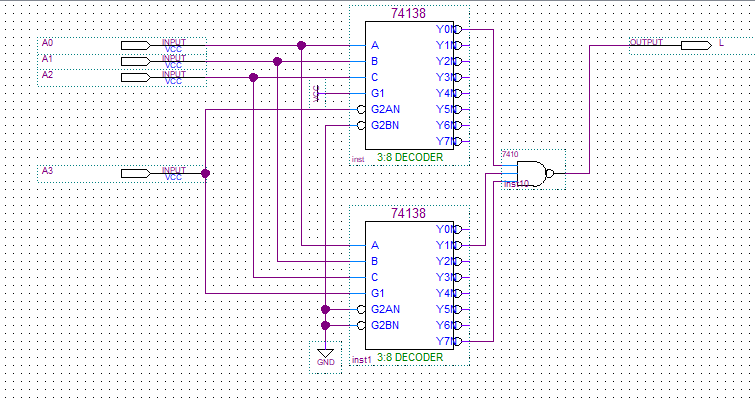
\includegraphics[width=0.95\textwidth]{密码锁电路.png}
    \caption{基于 74138 和与非门的密码锁原理图}
    \label{fig:lock_circuit}
\end{figure}

\subsection{全减器与密码锁联动}

将密码锁输出作为全减器模块的有效控制信号。当密码输入为 \texttt{1111} 时，控制信号有效，全减器输出差位和借位；当密码输入不正确时，控制信号无效，最终输出不作为有效减法结果。通过这种方式可验证组合逻辑模块的级联设计方法。

\begin{figure}[H]
    \centering
    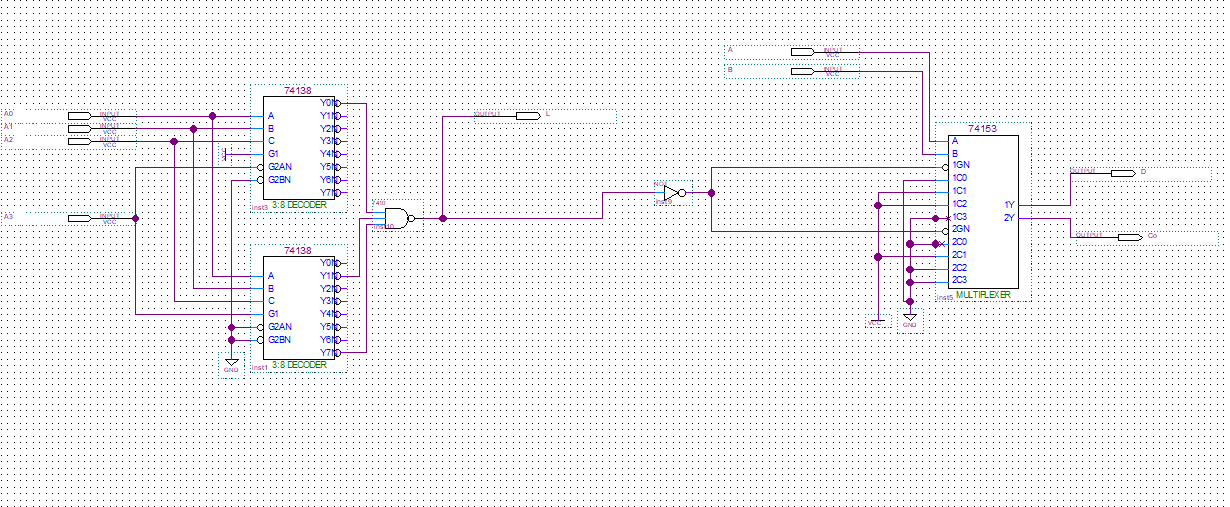
\includegraphics[width=0.95\textwidth]{最终电路.png}
    \caption{密码锁控制全减器工作的最终联动电路}
    \label{fig:final_circuit}
\end{figure}

\section{实验内容}

\subsection{工程创建与原理图输入}

启动 Quartus II，通过 \textbf{File $\rightarrow$ New Project Wizard} 创建实验二工程。在器件选择中指定 Cyclone V 系列的 \texttt{5CEBA4F23C7}，与 DE0 开发板保持一致。新建 Block Diagram/Schematic File 后，分别放置 74153、74138、7400、输入引脚和输出引脚，并按实验要求完成全减器、密码锁和最终联动电路的连接。

\subsection{一位全减器设计与仿真}

全减器部分使用 74153 的选择功能实现 $D$ 和 $C_o$ 两个输出。输入端 $A$、$B$ 和 $C_i$ 通过拨动开关给出，输出差位和借位连接到 LED。完成原理图后进行全编译，并建立波形仿真文件验证 8 种输入组合下输出是否与真值表一致。

\begin{figure}[H]
    \centering
    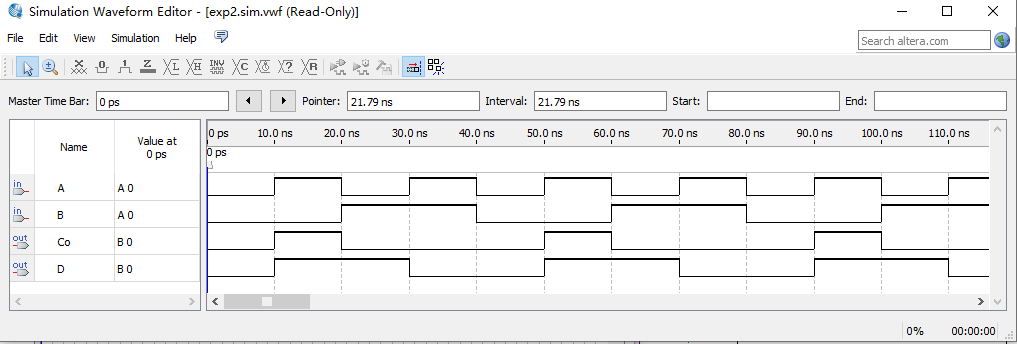
\includegraphics[width=\textwidth]{减法器仿真波形.png}
    \caption{一位全减器波形仿真结果}
    \label{fig:sub_wave}
\end{figure}

由图~\ref{fig:sub_wave} 可见，随着 $A$、$B$、$C_i$ 按不同组合变化，输出差位 $D$ 和借位 $C_o$ 能够对应全减器真值表变化，说明全减器模块逻辑正确。

\subsection{密码锁设计与仿真}

密码锁部分使用 74138 对输入状态进行译码，并使用与非门组合得到密码正确信号。设置密码为 \texttt{1111}，当密码输入满足该状态时，密码锁输出有效并驱动对应 LED；当输入为其他状态时，密码锁输出无效。

\begin{figure}[H]
    \centering
    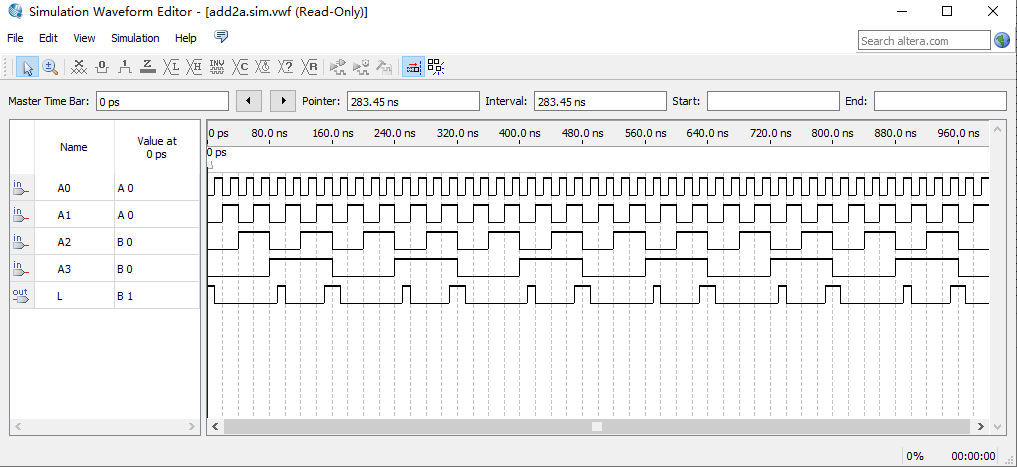
\includegraphics[width=\textwidth]{密码锁仿真波形.png}
    \caption{密码锁波形仿真结果}
    \label{fig:lock_wave}
\end{figure}

由图~\ref{fig:lock_wave} 可见，当输入密码为 \texttt{1111} 时，密码正确标志信号有效；其他输入状态下，标志信号保持无效，满足密码锁设计要求。

\subsection{联动电路设计与仿真}

在最终电路中，将密码锁输出接入全减器控制端。仿真时先改变密码输入，观察密码正确标志；再在密码正确状态下改变全减器输入，观察差位和借位是否正常变化。这样可以同时验证密码锁判断和全减器运算两个功能。

\begin{figure}[H]
    \centering
    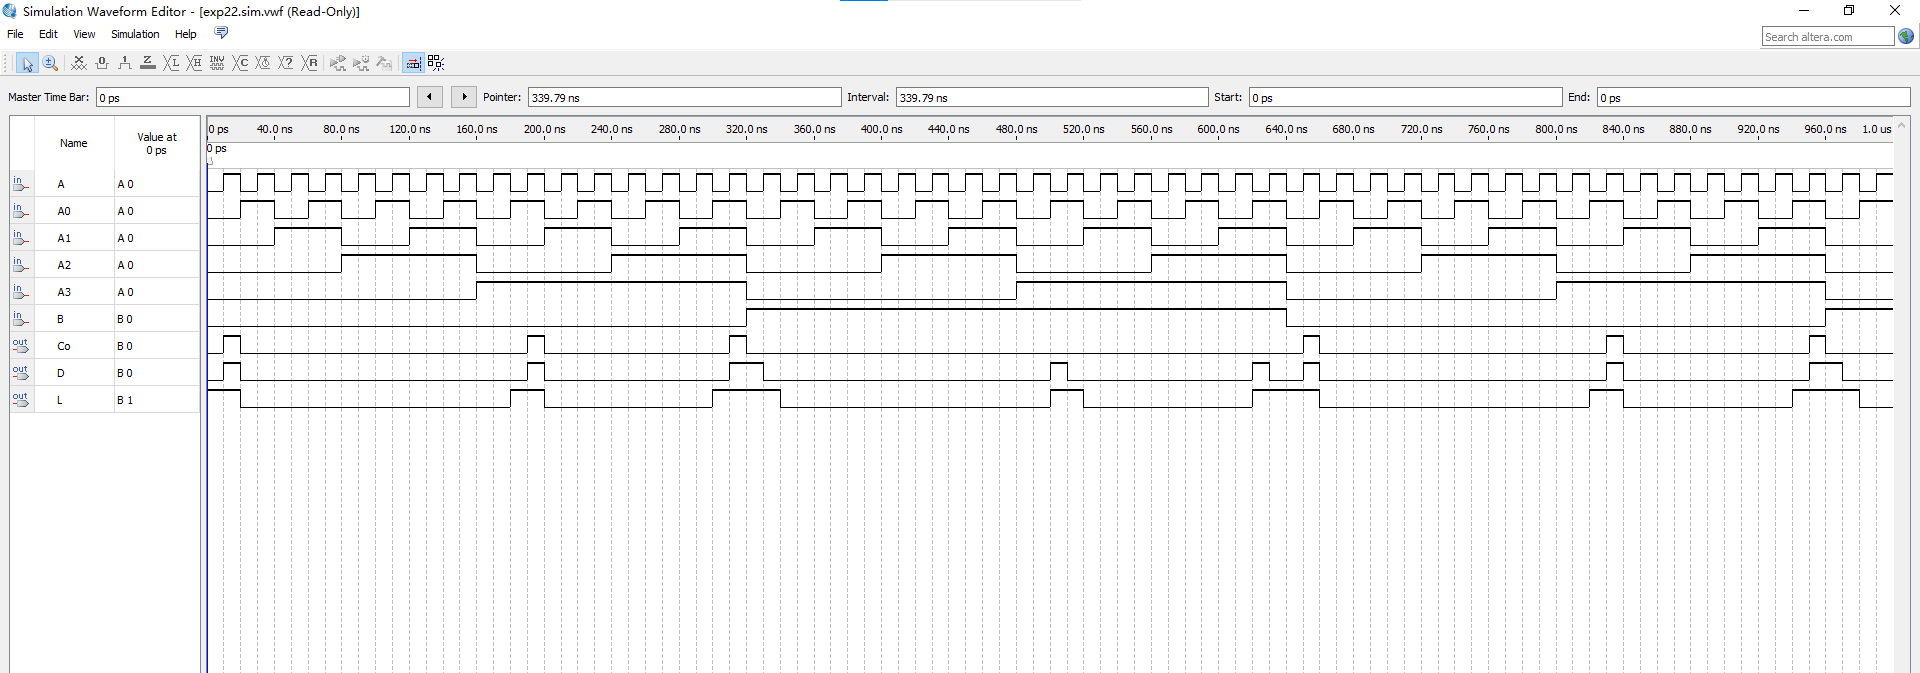
\includegraphics[width=\textwidth]{最终仿真波形.png}
    \caption{密码锁与全减器联动波形仿真结果}
    \label{fig:final_wave}
\end{figure}

由图~\ref{fig:final_wave} 可见，密码输入正确时，全减器输出能够随运算输入变化；密码输入不满足要求时，输出不表示有效运算结果，说明联动控制达到预期。

\subsection{引脚分配与下载验证}

根据实际原理图中的输入、输出端口，在 Quartus II 的 Pin Planner 中完成引脚锁定。由于本实验最终连接同时包含密码输入、全减器输入、密码正确指示和全减器输出，应以当前工程的端口命名和开发板实际接线为准，不在报告中固定列出通用引脚对照表。

完成引脚锁定后重新编译工程，生成可下载文件。连接 USB-Blaster 后，在 Quartus II Programmer 中选择 JTAG 模式并下载至开发板。通过拨动密码输入开关和全减器输入开关，观察对应 LED 状态，验证密码为 \texttt{1111} 时全减器能够正常工作。

\section{实验过程中的问题}

\begin{enumerate}
    \item 在使用 74138 设计密码锁时，需要注意 74138 输出为低有效信号，直接作为密码正确标志可能与 LED 显示或后级控制逻辑的有效电平不一致。因此在原理图连接时，应结合与非门统一信号极性，保证密码正确时控制信号有效。
    \item 在联动全减器和密码锁时，需要明确哪些输入属于密码锁、哪些输入属于全减器，避免仿真激励或引脚分配混淆。最终验证时应先确认密码锁输出正确，再观察全减器差位和借位是否随输入变化。
\end{enumerate}

\section{心得体会}

\begin{enumerate}
    \item 通过本次实验，我进一步理解了 74153 数据选择器和 74138 译码器在组合逻辑设计中的应用。相比直接用基本门电路搭建逻辑函数，中规模集成器件能够使电路结构更清晰，也更便于模块化设计。
    \item 本次实验将全减器和密码锁两个模块连接起来，使我认识到组合逻辑电路不仅要验证单个模块的真值关系，还需要关注模块之间控制信号的极性和有效条件。通过原理图输入、波形仿真和开发板验证，可以较完整地检查设计是否满足实验要求。
\end{enumerate}

\end{document}
